
\documentclass[tikz,border=5pt]{standalone}

% Core packages
\usepackage{amsmath,amssymb}
\usepackage{tikz}
\usepackage{tikz-cd}
\usepackage{pgfplots}
\usepackage{multicol}
\usepackage{xcolor}
\usepackage{caption}
\usepackage{float}
\usepackage{kotex}

% TikZ / PGF configuration
\usetikzlibrary{
  arrows.meta,
  calc,
  positioning,
  shapes.geometric,
  shapes.symbols,
  fit,
  backgrounds,
  patterns,
  matrix,
  intersections,
  decorations.pathmorphing,
  decorations.markings,
  angles,
  quotes
}
\pgfplotsset{compat=1.18}

% Reusable TikZ styles
\tikzset{
  >=stealth,
  line cap=round,
  line join=round,
  every picture/.style={line width=0.9pt},
  box/.style={draw, rounded corners, minimum width=2.8cm, minimum height=1.2cm, align=center},
  circlebox/.style={draw, circle, minimum size=1cm, align=center},
  arrow/.style={->, thick},
  dashedarrow/.style={->, thick, dashed},
  point/.style={circle, fill, inner sep=1.2pt},
  gridhelp/.style={help lines, gray!35},
  highlight/.style={fill=blue!10, draw=blue!60!black},
  3D/.style={
    x={(-0.60cm,-0.42cm)},
    y={(0.78cm,0cm)},
    z={(0cm,0.78cm)}
  }
}


\begin{document}

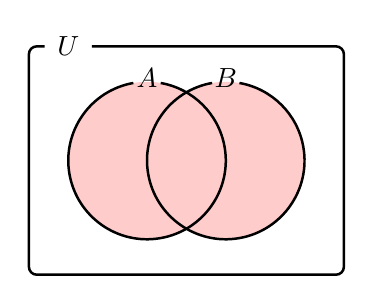
\begin{tikzpicture}[scale=1]
	% Draw the rectangle (universal set)
	\draw[rounded corners=1mm] (0.2, 2.7) -- (0, 2.7) -- (0, -0.2) -- (4, -0.2) -- (4, 2.7) -- (0.8, 2.7);
		
	\coordinate (centerA) at(1.5, 1.25);
	\coordinate (centerB) at(2.5, 1.25);
		
	% fill the circles A and B
	\fill[color=red!20] (centerA) circle (1);
	\fill[color=red!20] (centerB) circle (1);
		
	% draw the circle A as arc
	\draw (centerA) ++ (100:1) arc[start angle=100, end angle=440, radius=1];
	\draw (centerB) ++ (100:1) arc[start angle=100, end angle=440, radius=1];
		
	% Add labels
	\node at (1.5, 2.3) {$A$};
	\node at (2.5, 2.3) {$B$};
	\node at (0.5, 2.7) {$U$};
\end{tikzpicture}

\end{document}

